\documentclass[12pt]{article}
\usepackage[a4paper, margin=.30in]{geometry}
\usepackage{graphicx ,
            wrapfig,
            xcolor, 
            enumerate,
            amsmath,fontenc,tcolorbox
            }
\usepackage[european, straightvoltages,EFvoltages]{circuitikz}
\newcommand\headerMe[2]{\noindent{}#1\hfill#2}
\renewcommand{\thesection}{\Roman{section}}

\title{Leçon : }
\author{Zakaria HAOUZAN}
\date{\today}

\begin{document}
% headers --------------
\headerMe{Matière : Physique-Chimie}{Professeur : Zakaria HAOUZAN}\\
\headerMe{Unité : La Mécanique}{Établissement : Lycée SKHOR qualifiant}\\
\headerMe{Niveau : TCS}{Heure : 2H}\\

% ------Content ________
\begin{center}
  \Large{Leçon $N^{\circ}10$: \color{red} Association des conducteurs ohmiques }
\end{center}

\section{Etude d'un dipôle passif : le conducteur ohmique }

\subsection{Définition:}
On appelle dipôle tout composant électronique qui possède deux bornes.

Ce type de dipole ne peut pas fournir d'énergie électrique ,
mais seulement la consommer. (c'est un récepteur).

Les deux bornes du conducteur ohmique sont identiques.

On représente Le conducteur ohmique dans un circuit électrique par le symbole suivant :
  \begin{center}
  \begin{circuitikz}[european resistors]
      \draw (-0.5,0.1)node{A} (0,0)to[R,v<=$U_AB$,i=I, name=R] (2,0);
      \draw (2.2, 0) node{B};
    
  \end{circuitikz}
  \end{center}
R : est la résistance du conducteur ohmique ( l' unité de mesure de la résistance est l'ohm qu'on symbolise $\Omega $ et qui se mesure par un ohmmètre).

%\begin{wrapfigure}[4]{r}{0.39\textwidth}
    %\vspace{-1cm}
%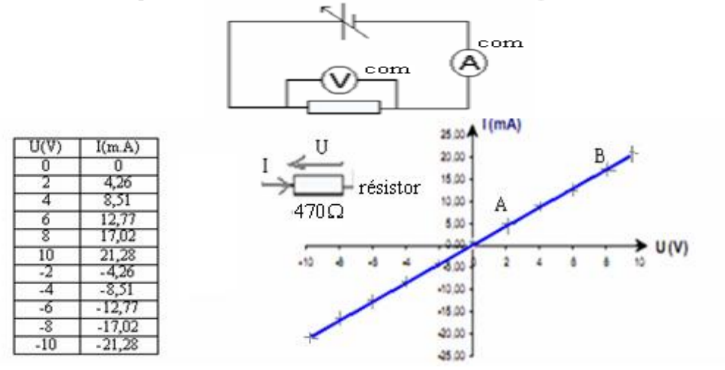
\includegraphics[width=0.39\textwidth]{./img/caracteristique_Resistor.png}
%\end{wrapfigure}


\subsection{Caractéristique d'un conducteur ohmique: }
On appelle caractéristique d'un conducteur ohmique la représentation graphique de la variation de la
tension U à ses bornes en fonction de l'intensité du courant qui le traverse: U=f(I).
Pour tracer la caractéristique d'un conducteur ohmique on utilise le montage suivant:
\begin{center}
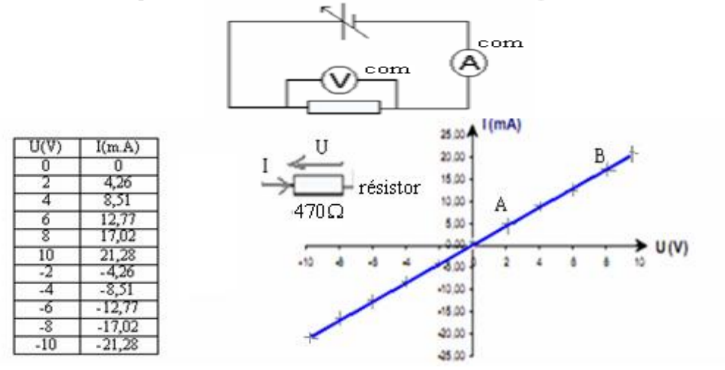
\includegraphics[width=0.7\textwidth]{./img/caracteristique_Resistor.png}
\end{center}

La caractéristique du conducteur ohmique est une droite qui passe par l'origine (droite lineaire.) .

Donc la tension aux bornes du conducteur ohmique est proportionnelle à l'intensité du courant qui le traverse : $U = R.I$

Cette relation traduit la loi d'ohm pour un conducteur ohmique.

Graphiquement la valeur de R se détermine par la méthode du coefficient directeur suivante : on choisi deux points
A et B de la droite U=f(I).

$R = \frac{\Delta{U}}{\Delta{I}} = \frac{U_B - U_A}{I_B - I_A} = \frac{8 - 2}{(17.02 - 4.26).10^{-3}A} = 470\Omega$

\subsection{Enoncé de la loi d'Ohm pour un conducteur ohmique : }

La tension UR aux bornes d'un conducteur ohmique est égale au produit de sa résistance R par l'intensité I
du courant qui le traverse : $U_R = R.I$

Dans la convention récepteur la tension UR aux bornes du conducteur ohmique et l'intensité I du courant qui le
traverse sont de sens contraires.
\begin{tcolorbox}{Remarque : }
 - La conductance G d'un conducteur ohmique est l'inverse de sa résistance: $G=\frac{1}{R}$ 
elle s'exprime en siemens (S). 

-Le rhéostat est une résistance variable.
\end{tcolorbox}

\subsection{Résistance d'un fil métallique:}
La résistance d'un fil métallique est donnée par la relation suivante: $R = \rho.\frac{l}{S}$
\\$l$  :la longueur du fil en (m).
\\S:la section du fil en $(m^2)$.
\\$\rho$ :la résistivité du matériau en $(\Omega.m)$

\section{Association des conducteurs ohmiques : }
\subsection{Association en série :}
On considère deux conducteurs ohmiques de résistances R1 et R2 montés en série.
Soit Re la résistance du conducteur ohmique équivalent qui peut les remplacer et jouer leur rôle.
\begin{center}
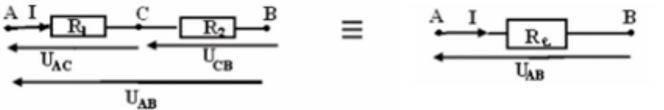
\includegraphics[width=0.5\textwidth]{./img/R_Serie.png}
\end{center}
En appliquant la loi d'additivité des tension : $U_{AB} = U_{AC} + U_{CB}$

On a  $U_{AC} = R_1.I$ et $U_{CB} = R_2.I$ En remplaçant $U_{AB} = I(R_1 + R_2)I$
donc $R_e = R_1 + R_2$
\begin{tcolorbox}{ }
Dans une association des conducteurs ohmiques en série , la résistance équivalent est égale à la somme des résistances $R_e = \sum R_i$
\end{tcolorbox}
  \subsection{Association en dérivation: }
On considère deux conducteurs ohmiques de résistances R1 et R2 montés en dérivation .
Soit Re la résistance du conducteur ohmique équivalent qui peut les remplacer et jouer leur rôle.
\begin{center}
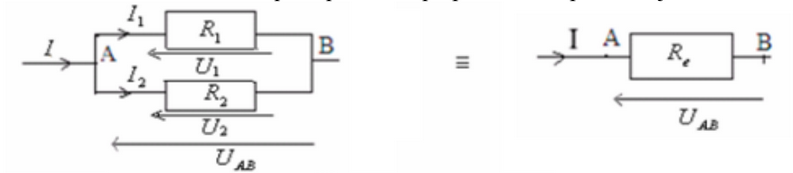
\includegraphics[width=0.5\textwidth]{./img/derivation.png}
\end{center}
En appliquant la loi des noeuds au point A : $I = I_1 + I_2$
  On a $I_1 = \frac{U_1}{R_1}$ et $I_2 = \frac{U_2}{R_2}$ donc $I = \frac{U_{AB}}{R_e}$
   
   alors $\frac{U_{AB}}{R_e} = \frac{U_1}{R_1} = \frac{U_2}{R_2}$

   Or dans un circuit en dérivation toutes les branches sont soumises à la même tension . $U_{AB} = U_1 = U_2$
   donc   $\frac{1}{R_e} = \frac{1}{R_1} = \frac{1}{R_2}$ alors  $G_e = G_1 + G_2$
\begin{tcolorbox}{ }
  Dans une association des conducteurs ohmiques en dérivation , la résistance équivalent est égale à la somme des conductances $\frac{1}{R_e} = \sum \frac{1}{R_i}$
\end{tcolorbox}

  \section{Utilisation des conducteurs ohmiques : }
\subsection{Diviseur de tension :}
Pour obtenir un générateur de tension variable à partir d'un générateur de tension continue on réalise un montage expérimental appelé diviseur de tension.

Pour avoir un diviseur de tension on monte un rhéostat en dérivation avec un générateur de tension continue .
\begin{center}
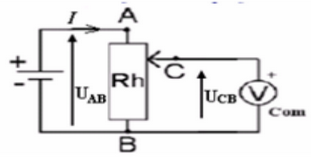
\includegraphics[width=0.2\textwidth]{./img/diviseur_Tension.png}
\end{center}
En déplaçant le curseur C du rhéostat ,l a tension de sortie UCB est variable.
\subsection {Relation du diviseur de tension :}
En appliquant la loi d'ohm : $U_{CB} = R_{CB}.I $ (1) et $U_{AB} = R_{AB}.I$ (2)

$\frac{2}{1}$ donc $\frac{U_{CB}}{U_{AB}} =\frac{R_{CB}}{R_{AB}} $
alors $$U_{CB} = \frac{R_{CB}}{R_{AB}}.U_{AB}$$

$R_{AB}$ : résistance totale du rhéostat.
$R_{CB}$ : une partie de la résistance totale du rhéostat qu'on peut faire varier en déplaçant le curseur.

\end{document}
